% !TeX root = main.tex

\section{Q1: 3R Manipulator}

The figure is shown below

\begin{figure}[h]
    \centering
    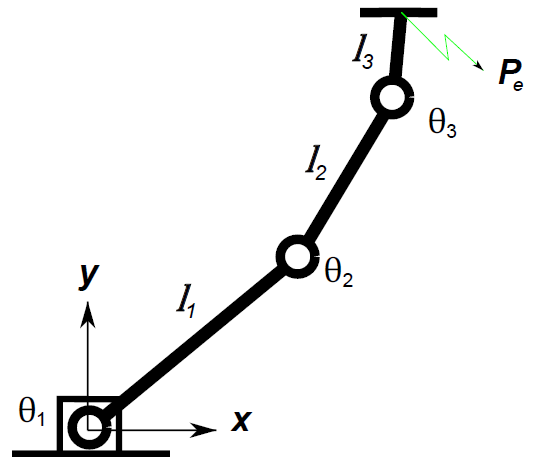
\includegraphics[width=0.4\textwidth]{3R-manip.png}
    \caption{Given 3R manipulator}
    \label{fig:q1-3r-manipulator}
\end{figure}

The forward kinematics for the manipulator shown in Figure \ref{fig:q1-3r-manipulator} is shown below

\begin{equation}
    \begin{bmatrix}
        x \\ y \\ \alpha
        \end{bmatrix}  = \begin{bmatrix}
        l_1 \cos(\theta_1) + l_2 \cos(\theta_1 + \theta_2) + l_3 \cos(\theta_1 + \theta_2 + \theta_3) \\
        l_1 \sin(\theta_1) + l_2 \sin(\theta_1 + \theta_2) + l_3 \sin(\theta_1 + \theta_2 + \theta_3) \\
        \theta_1 + \theta_2 + \theta_3
        \end{bmatrix} = \begin{bmatrix}
        l_1 c_1 + l_2 c_{12} + l_3 c_{123} \\
        l_1 s_1 + l_2 s_{12} + l_3 s_{123} \\
        \theta_1 + \theta_2 + \theta_3
        \end{bmatrix}
\end{equation}

Where $[x, y]$ is the position of end effector and $\alpha$ is the orientation in the plane (angle with X axis).

\subsection{Inverse Kinematics}

Here, given $\mathbf{x} = [x, y, \alpha]^\top$, we need to calculate $\theta_1$, $\theta_2$ and $\theta_3$. We first solve for the $\theta_1$ and $\theta_2$ by focusing on the pose of joint 3 as a 2R manipulator, then solve for $\theta_3$.

The inverse kinematics of a 2R manipulator can be derived using cosine rule and simple geometry as shown in Figure

\begin{figure}[h]
    \centering
    \begin{subfigure}[b]{0.3\textwidth}
        \centering
        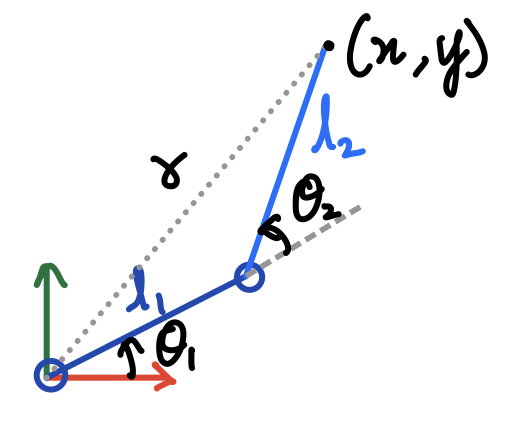
\includegraphics[width=\textwidth]{2R-manip.png}
        \caption{}
        \label{fig:sfig-2r-sub-3r}
    \end{subfigure}
    \begin{subfigure}[b]{0.3\textwidth}
        \centering
        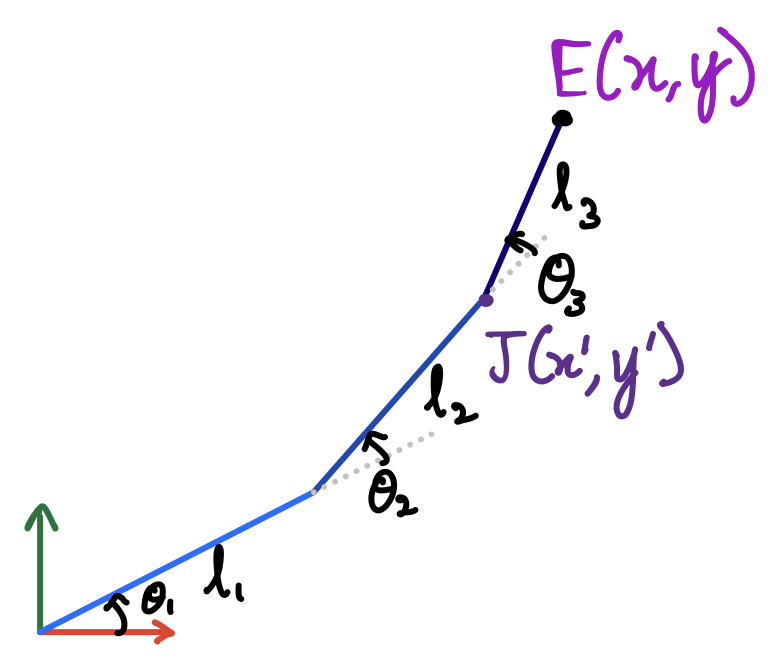
\includegraphics[width=\textwidth]{3R-manip-draw.PNG}
        \caption{}
        \label{fig:sfig-3r-manip}
    \end{subfigure}
    \begin{subfigure}[b]{0.3\textwidth}
        \centering
        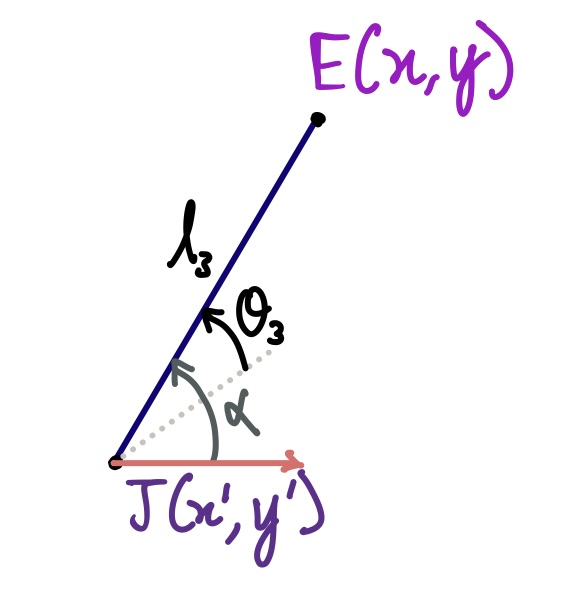
\includegraphics[width=\textwidth]{3R-j3ef.PNG}
        \caption{}
        \label{fig:sfig-3r-last-link}
    \end{subfigure}
    \caption{3R Manipulator breakdown}
    \label{fig:q1-3r-groupall}
    \small
        The figure \ref{sub@fig:sfig-2r-sub-3r} shows a 2R manipulator that can be visualized as a part of 3R manipulator till the third joint (3R manipulator shown in figure \ref{sub@fig:sfig-3r-manip}). The figure \ref{sub@fig:sfig-3r-last-link} shows the last link separately.
\end{figure}

\subsubsection*{IK of a 2R Manipulator}

From figure \ref{fig:sfig-2r-sub-3r}, it is clear that for a given 2R manipulator, one can derive the joint angles $\theta_1$ and $\theta_2$. The result is shown below

We first find $\theta_2$ using

\begin{align}
    r^2 &= x^2 + y^2 = \left ( l_1 + l_2 \cos (\theta_2) \right )^2 + \left ( l_2 \sin (\theta_2) \right )^2
    \nonumber \\
    &\Rightarrow x^2 + y^2 = l_1^2 + l_2^2+2l_1l_2\cos(\theta_2)
    \Rightarrow \cos(\theta_2) = \frac{x^2 + y^2 - l_1^2 - l_2^2}{2l_1l_2}
    \nonumber \\
    &\Rightarrow \theta_2 = \textup{acos} \left ( \frac{x^2 + y^2 - l_1^2 - l_2^2}{2l_1l_2} \right )
    \label{eq:2r-ik-t2}
\end{align}

For $\theta_1$, we do

\begin{align}
    \tan(\theta_1 + \beta) &= \frac{y}{x} &&
    \tan(\beta) = \frac{l_2 \sin(\theta_2)}{l_1 + l_2 \cos(\theta_2)} 
    \nonumber \\
    \Rightarrow \theta_1 + \beta &= \textup{atan2}(y, x) &&
    \beta = \textup{atan2} \left ( l_2 \sin(\theta_2) , l_1 + l_2 \cos(\theta_2) \right )
    \nonumber
\end{align}

This gives

\begin{equation}
    \Rightarrow \theta_1 = \textup{atan2}(y, x) - \textup{atan2} \left ( l_2 \sin(\theta_2) , l_1 + l_2 \cos(\theta_2) \right )
    \label{eq:2r-ik-t1}
\end{equation}

Note that $\theta_2$ is already found using Equation \ref{eq:2r-ik-t2}.

\subsubsection*{Extending to 3R}

From figure \ref{fig:sfig-3r-last-link}, we can estimate $J$ from $E$ (target end-effector position) using

\begin{equation}
    \begin{bmatrix}
        x' \\ y'
        \end{bmatrix} = \begin{bmatrix}
        x - l_3 \cos (\alpha) \\
        y - l_3 \sin (\alpha)
        \end{bmatrix}
    \label{eq:j3-fm-ef}
\end{equation}

We can now feed the point $[x', y']$ (instead of $[x, y]$) to the IK of 2R, that is equations \ref{eq:2r-ik-t1} and \ref{eq:2r-ik-t2} to get $\theta_1$ and $\theta_2$ respectively. Specifically, we get the inverse kinematics using the equations described below

\begin{align}
    & x_j = x - l_3 \cos(\alpha)
    & y_j = y - l_3 \sin(\alpha)
    \nonumber \\
    & \theta_2 = \textup{acos} \left ( \frac{x_j^2 + y_j^2 - l_1^2 - l_2^2}{2l_1l_2} \right )
    \label{eq:3r-ik-t2}
    \\
    & \theta_1 = \textup{atan2}(y_j, x_j) - \textup{atan2} \left ( l_2 \sin(\theta_2) , l_1 + l_2 \cos(\theta_2) \right )
    \label{eq:3r-ik-t1}
    \\
    && \theta_1 + \theta_2 + \theta_3 = \alpha
    \nonumber \\
    & \theta_3 = \alpha - \theta_1 - \theta_2
    \label{eq:3r-ik-t3}
\end{align}

Using equations \ref{eq:3r-ik-t1}, \ref{eq:3r-ik-t2}, and \ref{eq:3r-ik-t3} we can obtain the values for $\theta_1$, $\theta_2$ and $\theta_3$ for a 3R manipulator, given the end effector pose $[x, y, \alpha]$.

\subsection{Code implementation}

The figure \ref{fig:3r-ik-anim} shows different stages of an animation that includes moving the end effector along a straight line with a fixed orientation. The code for this is implemented in Appendix \ref{app:3r-ik-anim}.

The file \texttt{media/3R\_IK.mp4} includes a video for illustrating the animation.

\begin{figure}[ht]
    \centering
    \begin{subfigure}[b]{0.24\textwidth}
        \centering
        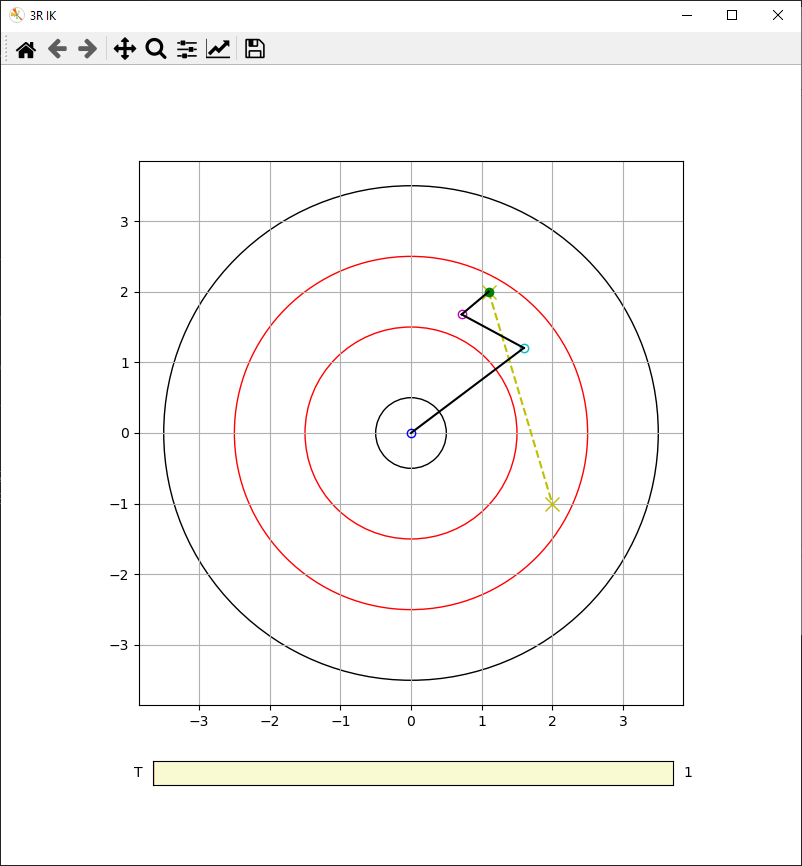
\includegraphics[width=\textwidth]{3R-Anim-1.png}
    \end{subfigure}
    \begin{subfigure}[b]{0.24\textwidth}
        \centering
        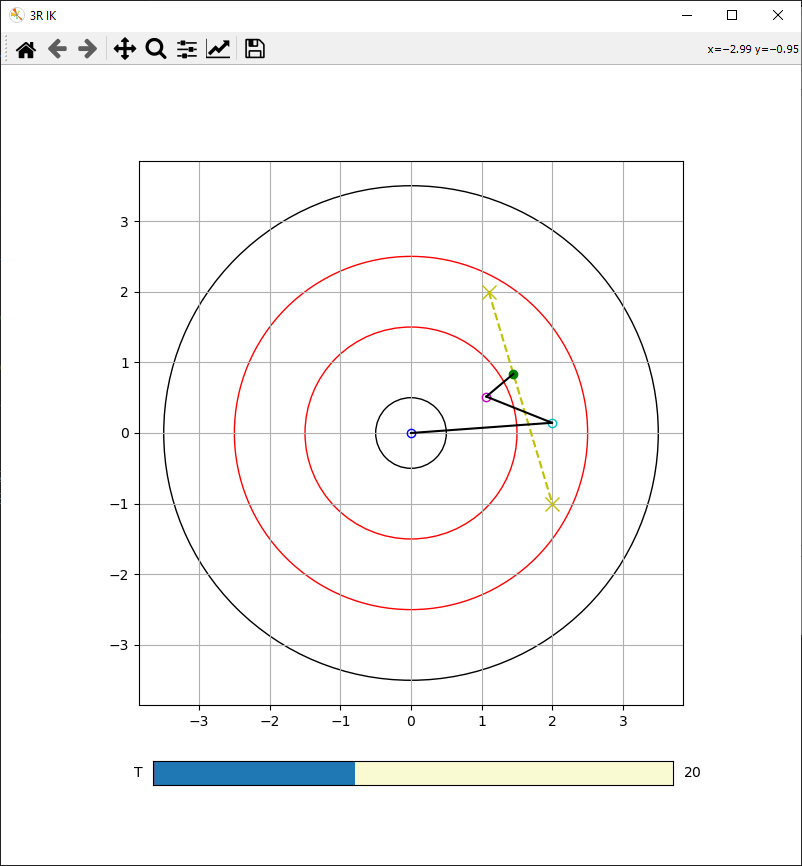
\includegraphics[width=\textwidth]{3R-Anim-2.png}
    \end{subfigure}
    \begin{subfigure}[b]{0.24\textwidth}
        \centering
        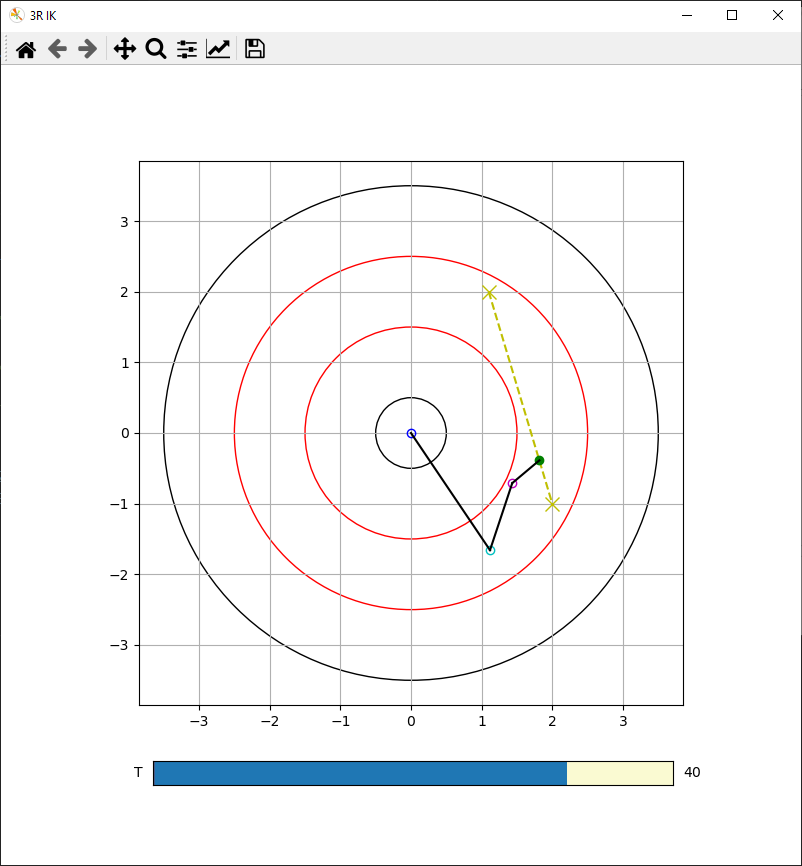
\includegraphics[width=\textwidth]{3R-Anim-3.png}
    \end{subfigure}
    \begin{subfigure}[b]{0.24\textwidth}
        \centering
        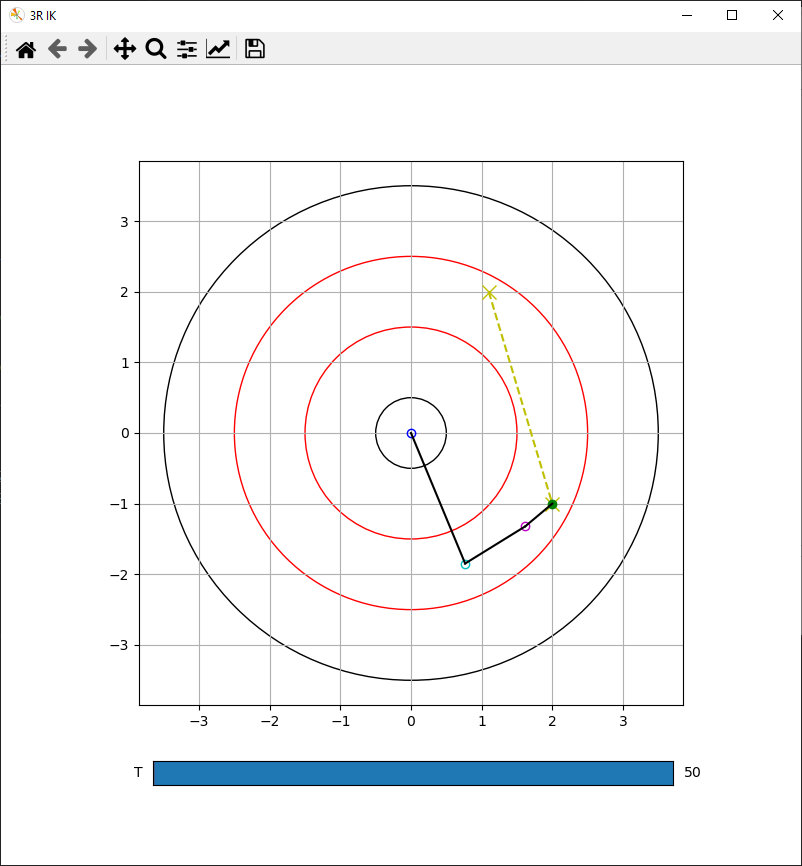
\includegraphics[width=\textwidth]{3R-Anim-4.png}
    \end{subfigure}
    \caption{Animations for 3R Inverse Kinematics}
    \label{fig:3r-ik-anim}
    \small
        A 3R manipulator tracing a path in the 2D plane, while maintaining the orientation. The code is implemented in Appendix \ref{app:3r-ik-anim}. The slider can be used move the end effector along the line. The region enclosed between the black circles is the \textit{reachable} workspace and the region enclosed between the red circles is the \textit{dexterous} workspace.
\end{figure}

\subsection{Singularity of 3R}

Singularity is a configuration when there is a locking. In such a case, changes in the joint coordinates do not change the end effector position (they bring no velocity). As the robot approaches the singularity, large changes in joint angles are needed to bring small changes to the end effector pose. This mathematically is when the jacobian (either the linear or angular velocity part) becomes zero.

The Jacobian of the 3R manipulator (like the one shown in figure \ref{fig:sfig-3r-manip}) is shown in equation \ref{eq:3r-jacobian}. The determinant of this jacobian matrix is shown in equation \ref{eq:3r-jacobian-det}. It is seen that the determinant of Jacobian is independent of the orientation of the end effector, it is varied only by the angle $\theta_2$.

\begin{align}
    \begin{bmatrix}
        x \\ y \\ \alpha
        \end{bmatrix} &= \begin{bmatrix}
        l_1 c_1 + l_2 c_{12} + l_3 c_{123} \\
        l_1 s_1 + l_2 s_{12} + l_3 s_{123} \\
        \theta_1 + \theta_2 + \theta_3
        \end{bmatrix}
    \nonumber \\
    \begin{bmatrix}
        \dot{x} \\ \dot{y} \\ \dot{\alpha}
        \end{bmatrix} &= \begin{bmatrix}
        -l_1 s_1-l_2 s_{12}-l_3 s_{123} & -l_2 s_{12}-l_3 s_{123} & -l_3 s_{123} \\
        l_1 c_1+l_2 c_{12}+l_3 c_{123} & l_2 c_{12}+l_3 c_{123} & l_3 c_{123} \\
        1 & 1 & 1
        \end{bmatrix} \begin{bmatrix}
        \dot{\theta_1} \\ \dot{\theta_2} \\ \dot{\theta_3}
        \end{bmatrix} 
    \nonumber \\
    \Rightarrow \mathbf{J} &= \begin{bmatrix}
        -l_1 s_1-l_2 s_{12}-l_3 s_{123} & -l_2 s_{12}-l_3 s_{123} & -l_3 s_{123} \\
        l_1 c_1+l_2 c_{12}+l_3 c_{123} & l_2 c_{12}+l_3 c_{123} & l_3 c_{123} \\
        1 & 1 & 1
        \end{bmatrix}
    \label{eq:3r-jacobian} \\
    \rightarrow \textup{det}(\mathbf{J}) &= l_1 l_2 \sin(\theta_1) \cos(\theta_1 + \theta_2) + l_1 l_2 \sin(\theta_1 + \theta_2) \cos(\theta_1) = l_1 l_2 \sin(\theta_2)
    \label{eq:3r-jacobian-det}
\end{align}

When $\sin(\theta_2) = 0$, then $\theta_2 = 0$ or $\theta_2 = \pi$. These are the singular configurations of the planar 3R manipulator. It can be seen that when such a configuration occurs, the end effector cannot move freely in all directions. It can only move on a loci of a fixed circle (whose radius depends on the orientation of the end effector).

When the orientation is fixed, then the joint angle $\theta_3$ can compensate to fix the orientation. This way, the circle may not be centered at origin, but will be offset (depending upon the link lengths). The end effector, will only be able to trace this circle, it cannot enter the dexterous workspace as shown in figure \ref{fig:3r-ik-anim}.
